\documentclass[a4paper]{article}

\usepackage[utf8]{inputenc}
\usepackage{polski}
\usepackage[polish]{babel}
\usepackage[margin=0.9in]{geometry}
\usepackage{lmodern}

\usepackage[pdftex]{graphicx}

\title{\textbf{Podsumowanie prac z projektu WDS - kwiecień 2015}}
\author{Marcin Ochman - 200546}
\date{}
\begin{document}


\begin{titlepage}
\begin{center}

 \newcommand{\HRule}{\rule{\linewidth}{0.5mm}}
%\includegraphics[width=0.15\textwidth]{./logo}~\\[1cm]

\textsc{\Large Projekt z Wizualizacji danych sensorycznych}\\[1cm]

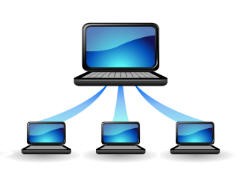
\includegraphics{network_icon}


\HRule \\[0.4cm]
{ \huge \bfseries \textit{Computer Monitor} - monitorowanie komputerów poprzez sieć.\\[0.4cm] }

{\huge \underline{\textit{Raport postępu prac }}}\\[0.5cm]


\LARGE 23.04.2015
\HRule \\[1.5cm]


\noindent
\begin{minipage}[t]{0.4\textwidth}
\begin{flushleft} \large
\emph{Autor:}\\
Marcin \textsc{Ochman}
\end{flushleft}
\end{minipage}%
\begin{minipage}[t]{0.4\textwidth}
\begin{flushright} \large
\emph{Prowadzący} \\
Dr inż. Bogdan \textsc{Kreczmer}
\end{flushright}
\end{minipage}


\end{center}
\end{titlepage}

\newpage

\tableofcontents
\listoffigures
\listoftables

\newpage

\section{Wprowadzenie}

W trakcie miesiąca zostało wykonanych wiele prac nad aplikacją.


\section{Lista wykonanych zadań w projekcie}

\section{Szczegółowy opis wykonanych zadań}

\subsection{Stworzenie zalążka aplikacji}

\subsubsection{Struktura folderów projektu}
\subsubsection{Architektura aplikacji}

\subsection{Biblioteka \textit{SystemMonitoringLib}}

\section{Następne zadania do wykonania}

\section{Podsumowanie}

\end{document}